\documentclass[tikz]{standalone}
\usepackage{pgfplots}
\pgfplotsset{compat=1.15}
\usepackage{mathrsfs}
\usetikzlibrary{arrows,calc}
\usepackage{tkz-euclide}
\pagestyle{empty}

\definecolor{AngleClr}{rgb}{0,0.39215686274509803,0}
\definecolor{ShapeClr}{rgb}{0.6,0.2,0}
\definecolor{SquareClr}{RGB}{250, 248, 217}

\begin{document}

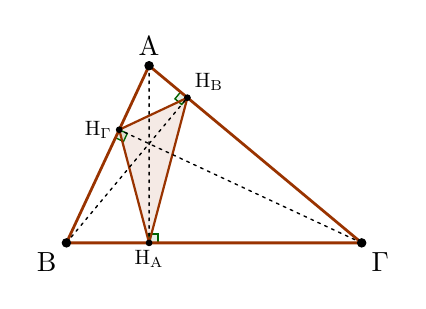
\begin{tikzpicture}[scale=.75]
\tkzSetUpLine[line width=1pt,color=black]
\tkzSetUpPoint[fill=black]

\tkzDefPoints{0/0/B,1.4/3/A,5/0/C}


\tkzDefPointBy[projection=onto B--C](A)\tkzGetPoint{HA}
\tkzDefPointBy[projection=onto A--C](B)\tkzGetPoint{HB}
\tkzDefPointBy[projection=onto A--B](C)\tkzGetPoint{HC}

\tkzFillPolygon[fill=ShapeClr,fill opacity=0.1](HA,HB,HC)
\tkzMarkRightAngles[line width=0.5pt, size=.15,color=AngleClr,fill=AngleClr,fill opacity=0.1](B,HC,C C,HA,A A,HB,B)

\tkzDrawPolygon[color=ShapeClr](A,B,C)
\tkzDrawPolygon[line width=0.8pt,color=ShapeClr](HA,HB,HC)

\tkzDrawPoints[size=3](A,B,C)
\tkzDrawPoints[size=2](HA,HB,HC)

\tkzDrawSegments[line width=0.5pt,color=black,dashed,dash pattern=on 1pt off 1.75pt](A,HA B,HB C,HC)

\tkzLabelPoint[above](A){$\mathrm{A}$}
\tkzLabelPoint[below left](B){$\mathrm{B}$}
\tkzLabelPoint[below right](C){$\mathrm{\Gamma}$}

\tkzLabelPoint[scale=0.75,below](HA){$\mathrm{H_A}$}
\tkzLabelPoint[scale=0.75,above right](HB){$\mathrm{H_B}$}
\tkzLabelPoint[scale=0.75,left](HC){$\mathrm{H_\Gamma}$}

\end{tikzpicture}

\end{document}
